%-----------------------------------------------------------------------------%
% \listoftables
\chapter{\babTiga}


%-----------------------------------------------------------------------------%
% \lipsum[6-6]

%-----------------------------------------------------------------------------%
\section{Kedudukan dan Koordinasi}
%-----------------------------------------------------------------------------%

Selama pelaksanaan kerja magang di PT Ganda Visi Jayatama, peran yang dijalankan berada dalam tim pengembangan sistem CHRIS (Concise Human Resources Information System) sebagai \textit{Backend Engineer Intern}. Tanggung jawab utamanya mencakup pengembangan dan pengujian \textit{Application Programming Interface} (API) yang digunakan oleh sistem, serta kolaborasi dengan anggota tim lainnya dalam penyusunan dan penyempurnaan fitur-fitur sistem kepegawaian berbasis \textit{web}.

\begin{figure}[H]
    \centering
    \fbox{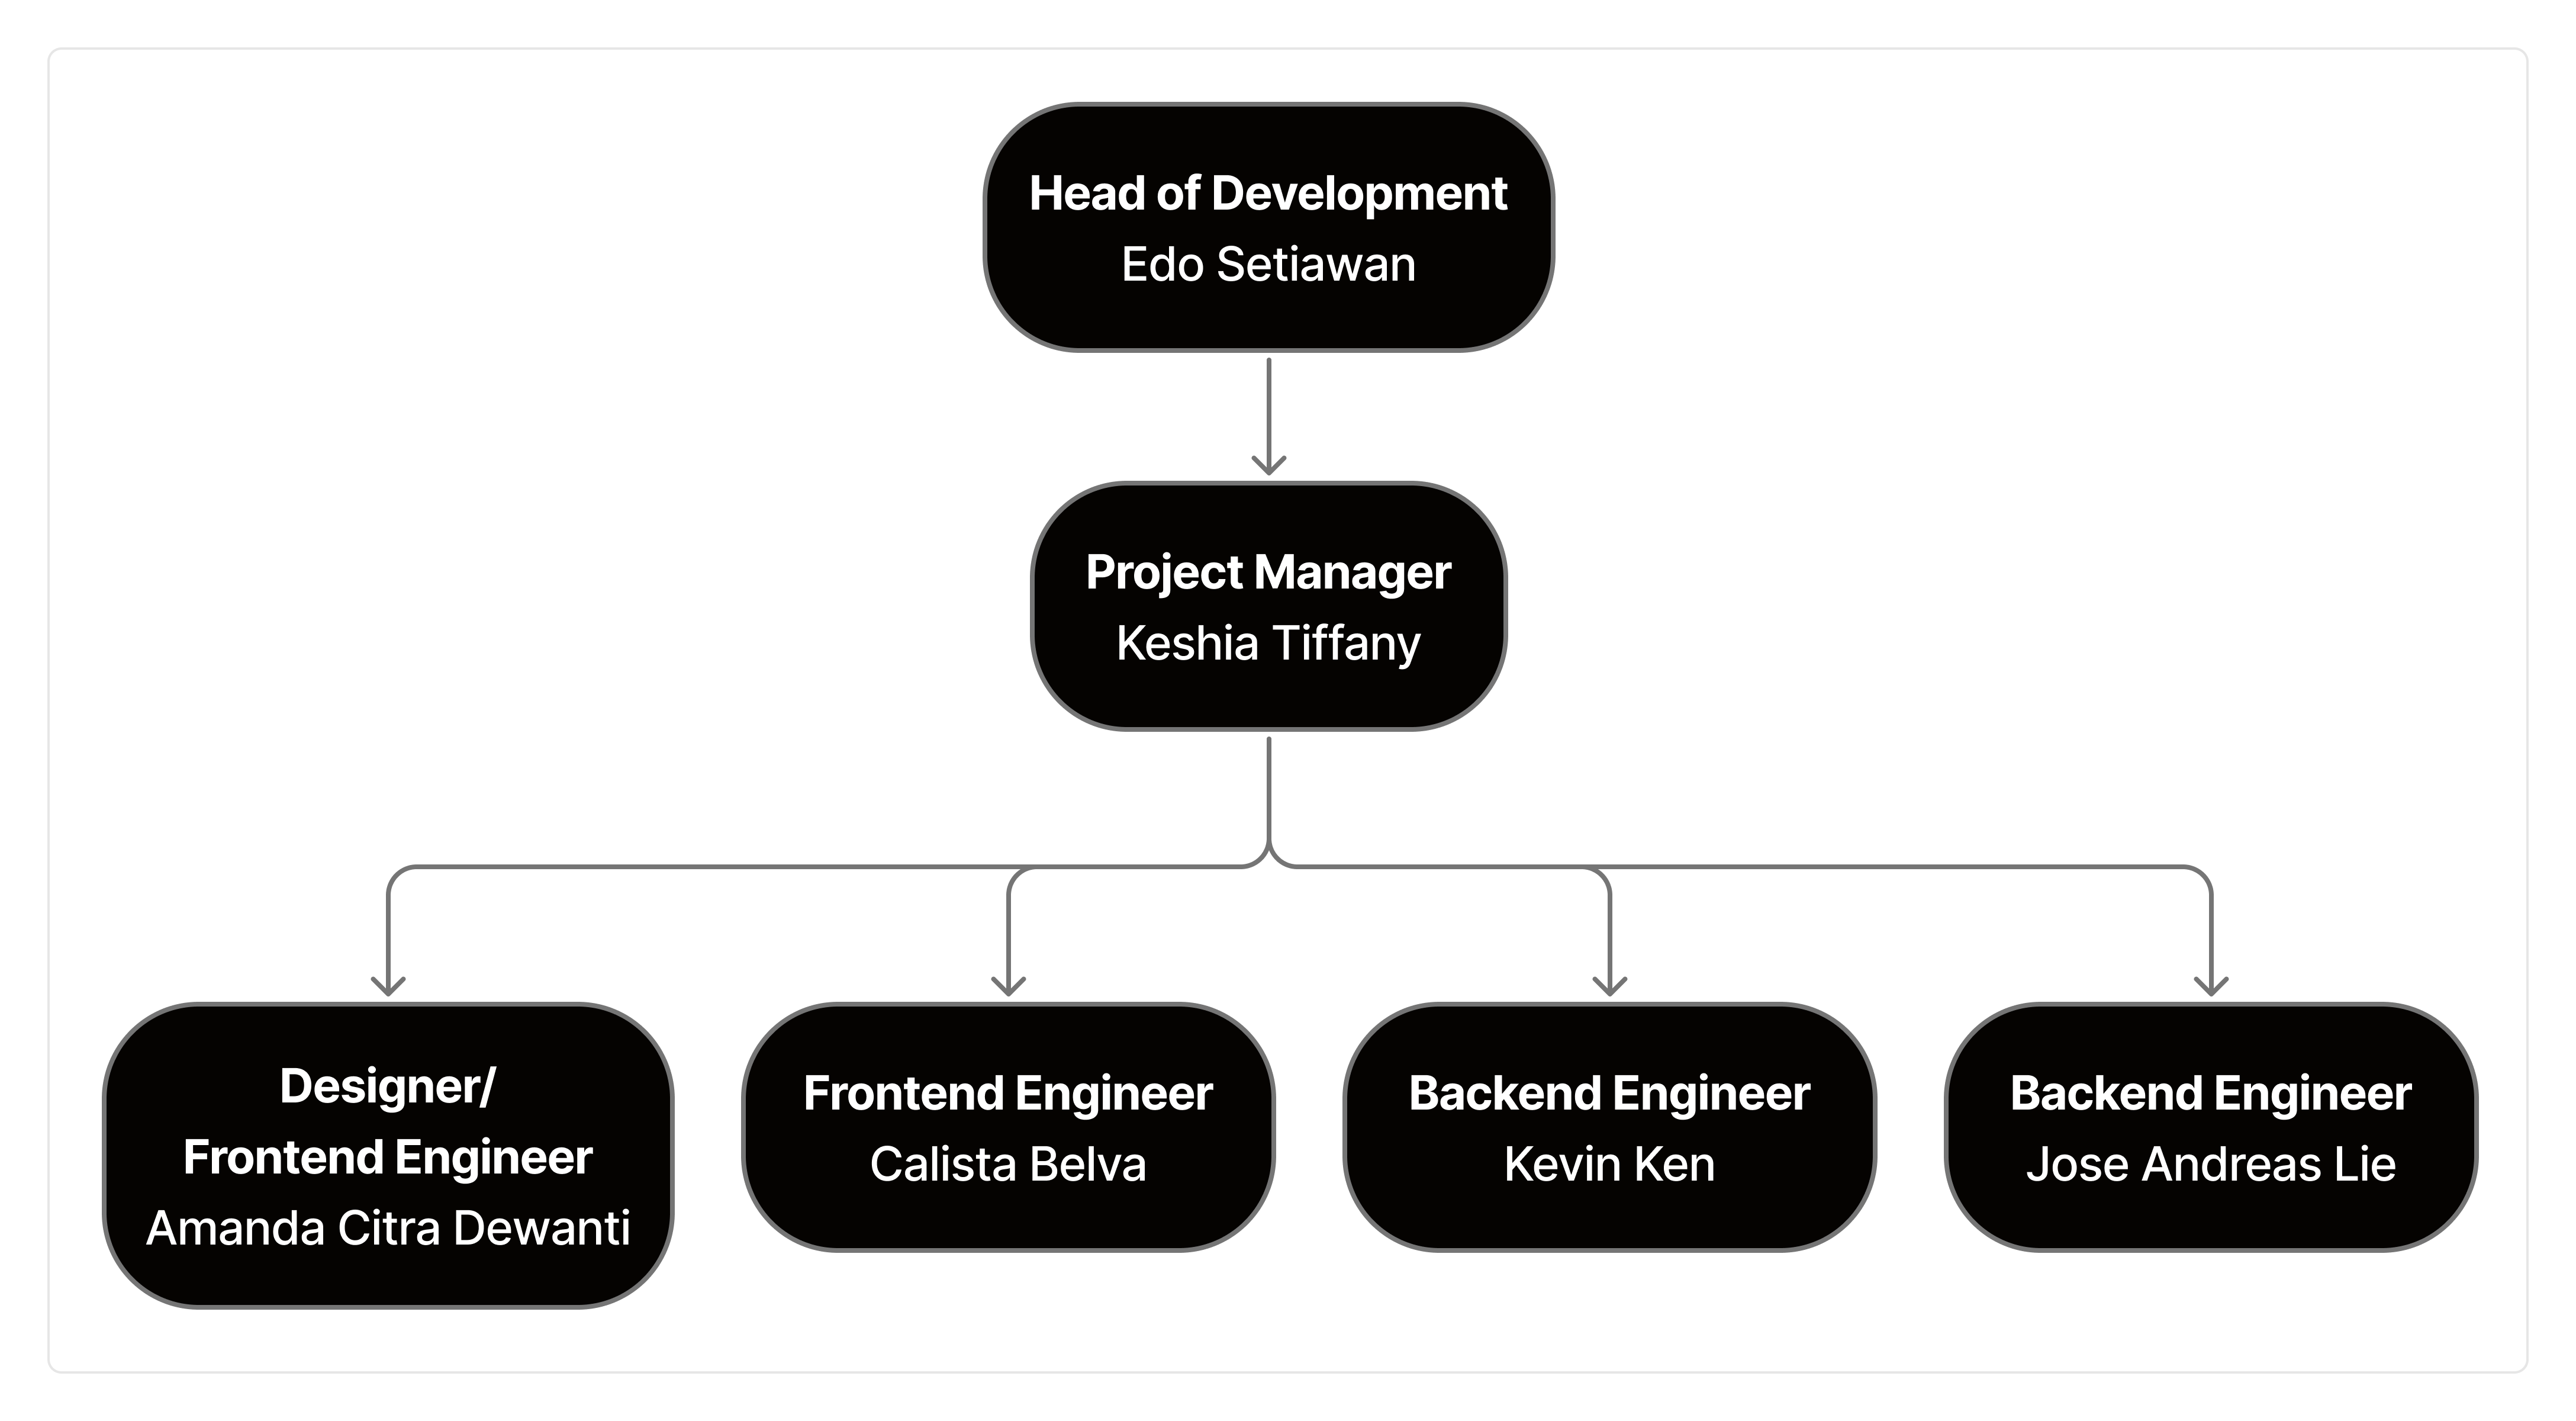
\includegraphics[width=0.8\textwidth]{assets/pics/fig_struktur_tim_chris.png}}
    \caption{Struktur Tim CHRIS}
    \label{fig:struktur_tim_CHRIS}
\end{figure}

Gambar \ref{fig:struktur_tim_CHRIS} merupakan struktur dari tim CHRIS yang terdiri dari sejumlah anggota dengan peran yang saling terintegrasi. Bimbingan diberikan oleh Bapak Edo Setiawan selaku \textit{Supervisor} sekaligus Head of Development, yang secara rutin melaksanakan evaluasi mingguan terhadap progres dan melakukan \textit{code review} atas hasil pengembangan \textit{backend}. Koordinasi teknis lebih lanjut dilaksanakan bersama Bapak Muhammad Alwin Alamsyah Handoko Putra selaku \textit{Backend Lead}, yang memimpin diskusi internal tim \textit{backend} setiap hari Jumat melalui \textit{Backend Internal Meeting}. Perencanaan serta distribusi tugas dikoordinasikan oleh \textit{Project Manager}, Ibu Keshia Tiffany, yang bertanggung jawab dalam pembagian \textit{backlog} kepada anggota tim, serta mengadakan sesi evaluasi pribadi (\textit{one-on-one}) dengan masing-masing anggota tim magang.

Dalam pengembangan tampilan antarmuka sistem, kolaborasi dilakukan bersama \textit{Designer} Amanda Citra Dewanti yang merancang desain akhir dari \textit{web}, serta dua \textit{Frontend Engineer Intern}, Amanda Citra Dewanti dan Calista Belva, yang membangun antarmuka \textit{web} menggunakan React. Sementara itu, pengembangan API menggunakan Express.js dan Node.js, serta pengelolaan basis data dengan PostgreSQL, dijalankan oleh dua Backend Engineer, yaitu Kevin Ken dan satu rekan lainnya dalam tim.

Seluruh kegiatan kerja magang dilakukan secara langsung di kantor (\textit{Work From Office}). Koordinasi dilakukan melalui \textit{daily standup} setiap pagi untuk melaporkan progres harian, menyampaikan rencana kerja, serta mendiskusikan kendala yang dihadapi. Setiap dua minggu sekali, tim juga melaksanakan \textit{sprint retrospective} untuk mengevaluasi hasil kerja dalam satu \textit{sprint} dan menentukan perbaikan serta target \textit{sprint} berikutnya. Penugasan proyek dikelola menggunakan \textit{platform} Jira (Atlassian) dalam bentuk \textit{backlog sprint} yang dibagikan kepada setiap anggota tim secara terstruktur dan terukur.


% \noindent \begin{align}\label{eq:garis}
% 	\cfrac{y - y_{1}}{y_{2} - y_{1}} = 
% 	\cfrac{x - x_{1}}{x_{2} - x_{1}}
% \end{align}

% \equ~\ref{eq:garis} di atas adalah persamaan garis. 
% \equ~\ref{eq:garis} dan \ref{eq:bola} sama-sama dibuat dengan perintah \bslash
% align. 
% Perintah ini juga dapat digunakan untuk menulis lebih dari satu persamaan. 

% \noindent \begin{align}\label{eq:bola}
% 	\underbrace{|\overline{ab}|}_{\text{pada bola $|\overline{ab}| = r$}} 
% 		= \sqrt[2]{(x_{b} - x_{a})^{2} + (y_{b} - y_{a})^{2} + 
% 				\vert\vert(z_{b} - z_{a})^{2}}
% \end{align}

%-----------------------------------------------------------------------------%
\section{Tugas yang Dilakukan}
% \label{sec:multiEqu}
%-----------------------------------------------------------------------------%

Selama pelaksanaan kerja magang di PT Ganda Visi Jayatama, terdapat tanggung jawab utama dalam satu proyek utama, yaitu pengembangan aplikasi \textit{Internal System}. Tugas-tugas yang dijalankan selama magang terbagi ke dalam beberapa aktivitas utama sebagai berikut:

\begin{enumerate}
    \item Mengembangkan API untuk kebutuhan aplikasi \textit{Internal System}, yang mencakup pembuatan fitur-fitur backend sesuai dengan spesifikasi fungsional.
    \item Melakukan dokumentasi terhadap API yang telah dikembangkan menggunakan \textit{platform} dokumentasi API, Apidog.
    \item Melakukan pengujian secara mandiri terhadap API yang dibuat untuk memastikan bahwa seluruh \textit{endpoint} berjalan sesuai dengan fungsinya, serta menangani \textit{error handling} dan validasi data.
\end{enumerate}


% %-----------------------------------------------------------------------------%
% \section{Membuat Tabel}
% %-----------------------------------------------------------------------------%
% Seperti pada gambar, tabel juga dapat diberi label dan caption. 
% Caption pada tabel terletak pada bagian atas tabel. 
% Contoh tabel sederhana dapat dilihat pada \tab~\ref{tab:tab1}.

% \begin{table}
% 	\centering
% 	\caption{Contoh Tabel}
% 	\label{tab:tab1}
% 	\begin{tabular}{l | c r}
% 		\hline
% 		& kol 1 & kol 2 \\ 
% 		\hline
% 		baris 1 & 1 & 2 \\
% 		baris 2 & 3 & 4 \\
% 		baris 3 & 5 & 6 \\
% 		jumlah  & 9 & 12 \\
% 		\hline
% 	\end{tabular}
% \end{table}

% Ada jenis tabel lain yang dapat dibuat dengan \latex~berikut 
% beberapa di antaranya. 
% Contoh-contoh ini bersumber dari 
% \url{http://en.wikibooks.org/wiki/LaTeX/Tables}

% \begin{table}
% 	\centering
% 	\caption{An example of rows spanning multiple columns}
% 	\label{row.spanning}
% 	\begin{tabular}{l l *{6}{c}}
%   		\hline % create horizontal line
%   		No & Name & \multicolumn{3}{c}{Week 1} & \multicolumn{3}{c}{Week 2} \\
%   		\cline{3-8} % create line from 3rd column till 8th column
%   		& & A & B & C & A & B & C\\
%   		\hline
%   		1 & Lala & 1 & 2 & 3 & 4 & 5 & 6\\
%   		2 & Lili & 1 & 2 & 3 & 4 & 5 & 6\\
%   		3 & Lulu & 1 & 2 & 3 & 4 & 5 & 6\\
%   		\hline
% 	\end{tabular}
% \end{table}

% \lipsum[43-44]

% \begin{table}
% 	\centering
% 	\caption{Penulisan judul tabel dan judul gambar adalah rata kiri kanan serta tidak dicetak tebal dan mengikuti cara penulisan kalimat (sentence case).}
% 	\label{column.spanning}
% 	\begin{tabular}{l c l}
% 		\hline
% 		Percobaan & Iterasi & Waktu \\
% 		\hline
% 		Pertama & 1 & 0.1 sec \\ \hline
% 		\multirow{2}{*}{Kedua} & 1 & 0.1 sec \\
%  		& 3 & 0.15 sec \\ 
%  		\hline
% 		\multirow{3}{*}{Ketiga} & 1 & 0.09 sec \\
%  		& 2 & 0.16 sec \\
%  		& 3 & 0.21 sec \\ 
%  		\hline
% 	\end{tabular}\\
% 	\vspace{1em}
% 	{\small Sumber: \url{http://en.wikibooks.org/wiki/LaTeX/Tables}}
% \end{table}


% \lipsum[45-46]

% \noindent \begin{align}\label{eq:matriks}	
% 	|\overline{a} * \overline{b}| &= |\overline{a}| |\overline{b}| \sin\theta 
% 		\\[0.2cm]
% 	\overline{a} * \overline{b} &=  
% 		\begin{array}{| c c c |}
% 			\hat{i} & x_{1} & x_{2} \\
% 			\hat{j} & y_{1} & y_{2} \\
% 			\hat{k} & z_{1} & z_{2} \\
% 		\end{array} \nonumber \\[0.2cm]
% 	&= \hat{i} \,
% 		\begin{array}{ | c c | }
% 			y_{1} & y_{2} \\
% 			z_{1} & z_{2} \\
% 		\end{array} 
% 	   + \hat{j} \,
% 		\begin{array}{ | c c | }
% 			z_{1} & z_{2} \\
% 			x_{1} & x_{2} \\
% 		\end{array} 
% 	   + \hat{k} \,	
% 		\begin{array}{ | c c | }
% 			x_{1} & x_{2} \\
% 			y_{1} & y_{2} \\
% 		\end{array}
% 		\nonumber
% \end{align}

% Pada \equ~\ref{eq:matriks} dapat dilihat beberapa baris menjadi satu bagian 
% dari \equ~\ref{eq:matriks}. 
% Sedangkan di bawah ini dapat dilihat bahwa dengan cara yang sama, \equ~
% \ref{eq:gabungan1}, \ref{eq:gabungan2}, dan \ref{eq:gabungan3} memiliki nomor 
% persamaannya masing-masing. 

% \noindent \begin{align}\label{eq:gabungan1}	
% 	\int_{a}^{b} f(x)\, dx + \int_{b}^{c} f(x) \, dx = \int_{a}^{c} f(x) \, dx
% 		\\\label{eq:gabungan2}
% 	\lim_{x \to \infty} \frac{f(x)}{g(x)} = 0 \hspace{1cm} 
% 		\text{jika pangkat $f(x)$ $<$ pangkat $g(x)$} \\\label{eq:gabungan3}
% 	a^{m^{a \, ^{n}\log b }} = b^{\frac{m}{n}}
% \end{align}



% Rumus \ref{eq:Precision} menunjukkan cara perhintungan \textit{Precision}.

% \addequation{\textit{Precision}}{%
% \begin{equation}  \label{eq:Precision}
%     Precision = \frac{TP}{TP+FP}
% \end{equation}
% }

% Rumus \ref{eq:Recall} menunjukkan cara perhitungan \textit{Recall}.

% \addequation{\textit{Recall}}{
% \begin{equation}  \label{eq:Recall}
%     Recall = \frac{TP}{TP+FN}
% \end{equation}

% }

% \addequation{\textit{F1 Score}}{%
% \begin{equation}  \label{eq:F1-score}
%     F1 Score = 2*\frac{Precision*Recall}{Precision+Recall}
% \end{equation}
% }

% -----------------------------------------------------------------------------%

\section{Uraian Pelaksanaan Magang}
% -----------------------------------------------------------------------------%
Pelaksanaan kerja magang diuraikan seperti pada Tabel~\ref{tab:tbl_uraian}.

\begin{center}
\begin{longtable}{|c|p{0.75\textwidth}|}
\caption{Pekerjaan yang dilakukan tiap minggu selama pelaksanaan kerja magang}
\label{tab:tbl_uraian} \\
\hline
\textbf{Minggu Ke -} & \textbf{Pekerjaan yang dilakukan} \\
\hline
\endfirsthead

\multicolumn{2}{c}%
{{\parbox{\textwidth}{\centering \tablename\ \thetable{} -- Pekerjaan yang dilakukan tiap minggu selama pelaksanaan kerja magang (lanjutan)}}} \\
\hline
\textbf{Minggu Ke -} & \textbf{Pekerjaan yang dilakukan} \\
\hline
\endhead

\hline \multicolumn{2}{|r|}{{Lanjut pada halaman berikutnya}} \\
\hline
\endfoot

\hline \hline
\endlastfoot

1 & Mempelajari boilerplate backend dan mulai mengembangkan API untuk Employee Status pada sistem CHRIS. \\
\hline
2 & Melanjutkan pengembangan dan penyempurnaan API Employee Status serta melakukan validasi ulang pada form Employee di sistem CHRIS. \\
\hline
3 & Melakukan revisi minor pada API employee form, menyelesaikan tabel User dan Employee Status, serta berpartisipasi dalam Sprint Retro. \\
\hline
4 & Mengembangkan fitur pagination untuk berbagai modul (User, Leave, Attendance), membuat API form pengajuan cuti, serta melakukan code review dan diskusi dalam monthly meeting. \\
\hline
5 & Fokus pada revisi dan pengembangan API perizinan cuti, integrasi dengan frontend, serta showcase sistem CHRIS dan implementasi pagination untuk Leave Types. \\
\hline
6 & Melakukan revisi dan filtering pada Leave Permit Dashboard, menambahkan fitur cancel, serta aktif dalam code review dan weekly meeting tim backend. \\
\hline
7 & Melakukan berbagai pengujian dan UAT untuk Leave Management, membangun sistem tree berbasis jabatan untuk izin, serta menangani revisi migrasi dan API CHRISM (CHRIS Mobile). \\
\hline
8 & Mengembangkan sistem hierarki supervisi berbasis tree, menerapkan biometrik pada login API, dan mulai membangun user report summary API serta mempersiapkan People Report. \\
\hline
9 & Fokus pada penyempurnaan fitur User Report, termasuk penambahan filter tanggal dan perbaikan minor, serta melakukan hashing biometrik dan refactor pada dashboard Leave Permit. \\
\hline
10 &  Memulai riset intensif terkait sistem Payroll dan skema tabelnya, membuat dokumentasi di Apidog.\\
\hline
11 &  Melanjutkan pengembangan API Payroll berdasarkan hasil riset skema tabel, memperbarui dokumentasi di Apidog, serta mengikuti kegiatan Backlog Planning dan Sprint Closing.\\
\hline
12 &  Fokus pada pengembangan lanjutan API Payroll termasuk fitur Create, Get, Update, dan Delete, serta mulai menangani logika data untuk User Allowances.\\
\hline
13 &  Melanjutkan secara intensif pengembangan API Payroll khusus untuk pengelolaan dan perhitungan Each User Allowances secara berkelanjutan sepanjang minggu.\\
\hline
14 &  Mulai mengembangkan dan menyempurnakan Salary Slip APIs serta melakukan bugfix dan refactor pada User Allowance dan konfigurasi Payroll untuk integrasi dengan frontend.\\
\hline
15 &  Menambahkan fitur penghapusan User Allowance, memperbaiki konfigurasi endpoint Payroll, dan membuat API gabungan untuk manajemen detail user, payroll, serta tunjangan.\\
\hline
16 &  Melanjutkan integrasi Salary Slip dengan frontend serta melakukan pengujian menyeluruh terhadap modul Payroll, Allowance, dan Salary Slip.\\
\hline
17 &  Melakukan perbaikan pada logika dan pagination Salary Slip serta Payroll Config, merevisi sistem, dan menyiapkan internal report serta showcase Payroll.\\
\hline

\end{longtable}
\end{center}

% \begin{table}
% 	\centering
% 	\caption{ Pekerjaan yang dilakukan tiap minggu selama pelaksanaan kerja magang}
% 	\label{tbl_uraian}
% 	\begin{tabular}{|c | p{0.75\textwidth}| }
% 		\hline
% 		Minggu Ke - & Pekerjaan yang dilakukan \\
% 		\hline
% 		1 & 
% 		Mempelajari boilerplate backend dan mulai mengembangkan API untuk Employee Status pada sistem CHRIS.\\
% 		\hline
%  		2 & 
% 		Melanjutkan pengembangan dan penyempurnaan API Employee Status serta melakukan validasi ulang pada form Employee di sistem CHRIS.\\
% 		\hline
%  		3 & 
% 		Melakukan revisi minor pada API employee form, menyelesaikan tabel User dan Employee Status, serta berpartisipasi dalam Sprint Retro. \\
%  		\hline
%  		4 & 
% 		Mengembangkan fitur pagination untuk berbagai modul (User, Leave, Attendance), membuat API form pengajuan cuti, serta melakukan code review dan diskusi dalam monthly meeting \\
%  		\hline
%  		5 & 
% 		Fokus pada revisi dan pengembangan API perizinan cuti, integrasi dengan frontend, serta showcase sistem CHRIS dan implementasi pagination untuk Leave Types.\\
%  		\hline
%  		6 & 
% 		Melakukan revisi dan filtering pada Leave Permit Dashboard, menambahkan fitur cancel, serta aktif dalam code review dan weekly meeting tim backend.\\
%  		\hline
%  		7 & 
% 		Melakukan berbagai pengujian dan UAT untuk Leave Management, membangun sistem tree berbasis jabatan untuk izin, serta menangani revisi migrasi dan API CHRISM (CHRIS Mobile).\\
%  		\hline
%  		8 & Mengembangkan sistem hierarki supervisi berbasis tree, menerapkan biometrik pada login API, dan mulai membangun user report summary API serta mempersiapkan People Report.\\
%  		\hline
%  		9 & \\
%  		\hline
%  		10 & \\
%  		\hline
% 	\end{tabular}
% \end{table}



%-----------------------------------------------------------------------------%
\section{Pengumpulan dan Analisis Kebutuhan}
%-----------------------------------------------------------------------------%
Kebutuhan sistem dalam proyek ini diperoleh melalui koordinasi langsung dengan \textit{supervisor} dan tim \textit{backend internal}. Sebagian besar \textit{requirement} ditentukan secara iteratif berdasarkan kebutuhan bisnis dan sprint mingguan yang telah direncanakan oleh tim. Proses pengumpulan \textit{requirement} dilakukan melalui diskusi teknis, \textit{retrospective meeting}, dan \textit{task assignment} harian.

Berikut ini adalah uraian \textit{requirement} utama yang berhasil diidentifikasi dan diimplementasikan dalam proyek selama masa kerja praktik.
%-----------------------------------------------------------------------------%
\subsubsection{Refaktor User Management dan Validasi Data}

Pengembangan dimulai dengan perbaikan sistem \textbf{User Management}, termasuk validasi \textit{form input} dan \textit{refactor} struktur tabel seperti \textbf{user} dan \textbf{employment status}. Hal ini bertujuan untuk memastikan integritas data pengguna dan kemudahan pengelolaan melalui backend maupun frontend.
%-----------------------------------------------------------------------------%
\subsubsection{Optimalisasi Leave Permit}

Modul \textbf{Leave Permit} dikembangkan agar lebih efisien dan intuitif. Perubahan meliputi \textit{refactor} pada proses \textit{form submission}, penambahan tombol pembatalan (\textit{cancel}) pengajuan cuti, serta tampilan daftar cuti untuk atasan. Fitur-fitur ini dirancang agar mencerminkan alur persetujuan yang realistis dan terstruktur.
%-----------------------------------------------------------------------------%
\subsubsection{Implementasi Pagination}

Untuk mendukung jumlah data yang besar, sistem pagination ditambahkan pada beberapa modul utama seperti User, Leave, dan Attendance. Hal ini dilakukan guna menjaga performa dan kenyamanan pengguna.
%-----------------------------------------------------------------------------%
\subsubsection{Pengembangan Sistem Hierarki}

Dibuat fungsi \textit{tree hierarchy} berdasarkan struktur jabatan untuk mendukung fitur-fitur seperti izin cuti (\textit{accept}/\textit{reject}) dan tampilan dashboard atasan. Fungsi ini menjadi dasar logika akses dan pengelolaan hubungan antar pegawai.
%-----------------------------------------------------------------------------%
\subsubsection{Modul Payroll}

Modul \textbf{Payroll} dikembangkan untuk menghasilkan slip gaji setiap bulannya yang dihitung berdasarkan tunjangan. Termasuk di dalamnya pengembangan API untuk CRUD data payroll, penyusunan salary slip, dan integrasi dengan frontend.
% ---------------------------------------------------------------------------------%
\section{Perancangan dan Pengembangan Sistem}
% ---------------------------------------------------------------------------------%
Bagian ini menjelaskan perancangan dan pengembangan sistem yang mencakup struktur basis data dan alur sistem untuk fitur-fitur yang dikembangkan selama masa kerja praktik.

\subsection{Payroll}
Modul \textit{Payroll} merupakan salah satu fitur utama dalam sistem CHRIS\@. Modul ini bertujuan untuk mengelola data penggajian pegawai, termasuk perhitungan gaji berdasarkan tunjangan yang telah ditentukan.

\subsubsection{Diagram ERD Payroll}
\begin{figure}[H]
    \centering
    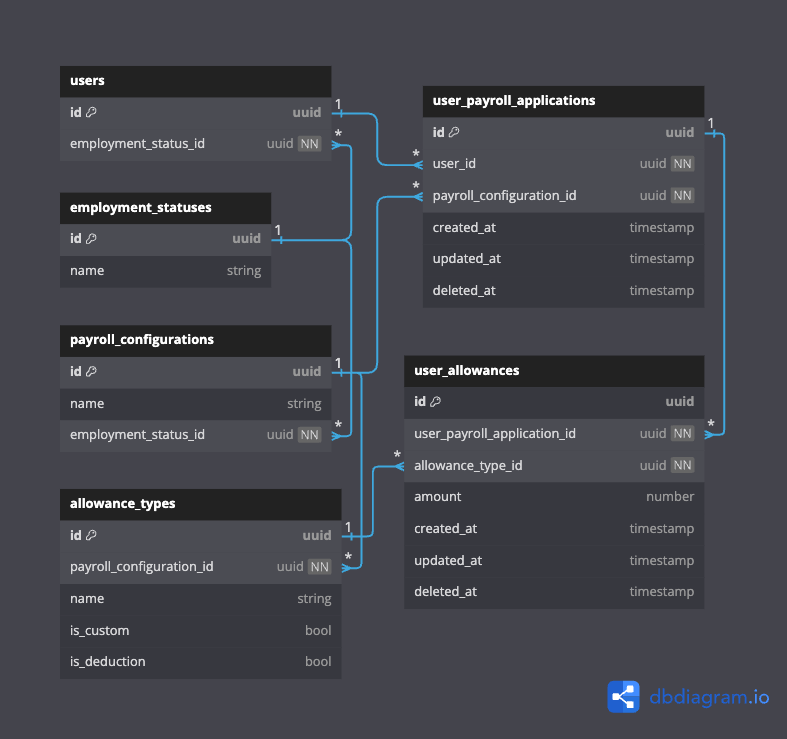
\includegraphics[width=0.8\textwidth]{assets/pics/fig_erd_payroll.png}
    \caption{Diagram ERD untuk modul Payroll}
    \label{fig:erd_payroll}
\end{figure}

Struktur basis data untuk modul Payroll terdiri dari beberapa tabel utama yang saling berhubungan. Berikut adalah penjelasan singkat mengenai tabel-tabel tersebut:
\begin{itemize}
    \item \textbf{User}: Tabel ini menyimpan data pegawai yang mencakup informasi pribadi, status kepegawaian, dan referensi ke konfigurasi penggajian yang digunakan.
    \item \textbf{Employment Status}: Tabel ini menyimpan data status kepegawaian yang digunakan sebagai referensi pada berbagai modul dalam sistem, salah satunya adalah modul \textit{Payroll}.
    \item \textbf{Payroll Configuration}: Tabel ini menyimpan konfigurasi penggajian yang mencakup nama, status kepegawaian, dan tunjangan yang berlaku. Setiap konfigurasi dapat memiliki beberapa tunjangan yang terkait.
    \item \textbf{Allowances Types}: Tabel ini menyimpan jenis-jenis tunjangan yang tersedia pada payroll configuraion yang telah dibuat, dan juga tunjangan tambahan untuk pegawai tertentu. Setiap jenis tunjangan memiliki nama, dan tipe (tunjangan atau potongan).
    \item \textbf{User Payroll Application}: Tabel ini menyimpan data Payroll yang telah diisi oleh \textit{Superadmin} untuk setiap pegawai.
    \item \textbf{User Allowances}: Tabel ini menyimpan data tunjangan spesifik untuk setiap pegawai. Tabel ini berisi informasi mengenai jenis tunjangan, jumlah, dan referensi ke pegawai yang bersangkutan.
\end{itemize}

\subsubsection{Alur Sistem Payroll}
Alur sistem \textit{Payroll} diawali dengan pembuatan data \textit{Payroll Configuration}, yang mencakup nama konfigurasi, status kepegawaian (\textit{Employment Status}), serta daftar tunjangan (\textit{Allowances}) yang berlaku. Setelah konfigurasi dibuat, \textit{Superadmin} melanjutkan ke modul \textit{User Management} untuk mengatur data gaji setiap pegawai secara individual.

Dalam modul \textit{User Management}, \textit{Superadmin} memilih \textit{Payroll Configuration} berdasarkan status kepegawaian pengguna, mengisi besaran gaji pokok, serta melengkapi jumlah masing-masing tunjangan yang ditetapkan. Selain itu, \textit{Superadmin} juga dapat menambahkan tunjangan (\textit{allowance}) atau potongan (\textit{deduction}) khusus yang hanya berlaku bagi pengguna tersebut, guna menyesuaikan skema gaji secara fleksibel.

Setelah data selesai disimpan, \textit{Superadmin} dapat mengakses modul \textit{Salary Slip} untuk melakukan finalisasi gaji. Finalisasi ini memungkinkan pengecekan akhir terhadap rincian gaji sebelum tanggal gajian. Di PT Ganda Visi Jayatama, proses penggajian dilakukan setiap tanggal 25, sehingga proses finalisasi disarankan dilakukan pada tanggal 24 setiap bulannya. Setelah tanggal 25, data tidak dapat lagi diubah.

Pegawai yang telah memiliki data gaji terverifikasi dapat melihat slip gaji mereka masing-masing pada halaman \textit{Salary Slip} dan mengunduhnya dalam format PDF.

\paragraph{Payroll Configuration}

Pada Gambar \ref{create_payroll_config}, \ref{update_payroll_config}, dan \ref{delete_payroll_config} merupakan alur sistem untuk Payroll Configuration yang dimulai dari pembuatan konfigurasi penggajian, di mana \textit{Superadmin} membuat konfigurasi baru dengan mengisi nama konfigurasi, status kepegawaian, dan daftar tunjangan (\textit{Allowances}) yang berlaku. Setelah itu, \textit{Superadmin} dapat mengakses modul \textit{User Management} untuk mengatur data gaji setiap pegawai.
\begin{figure}[H]
    \centering
    \fbox{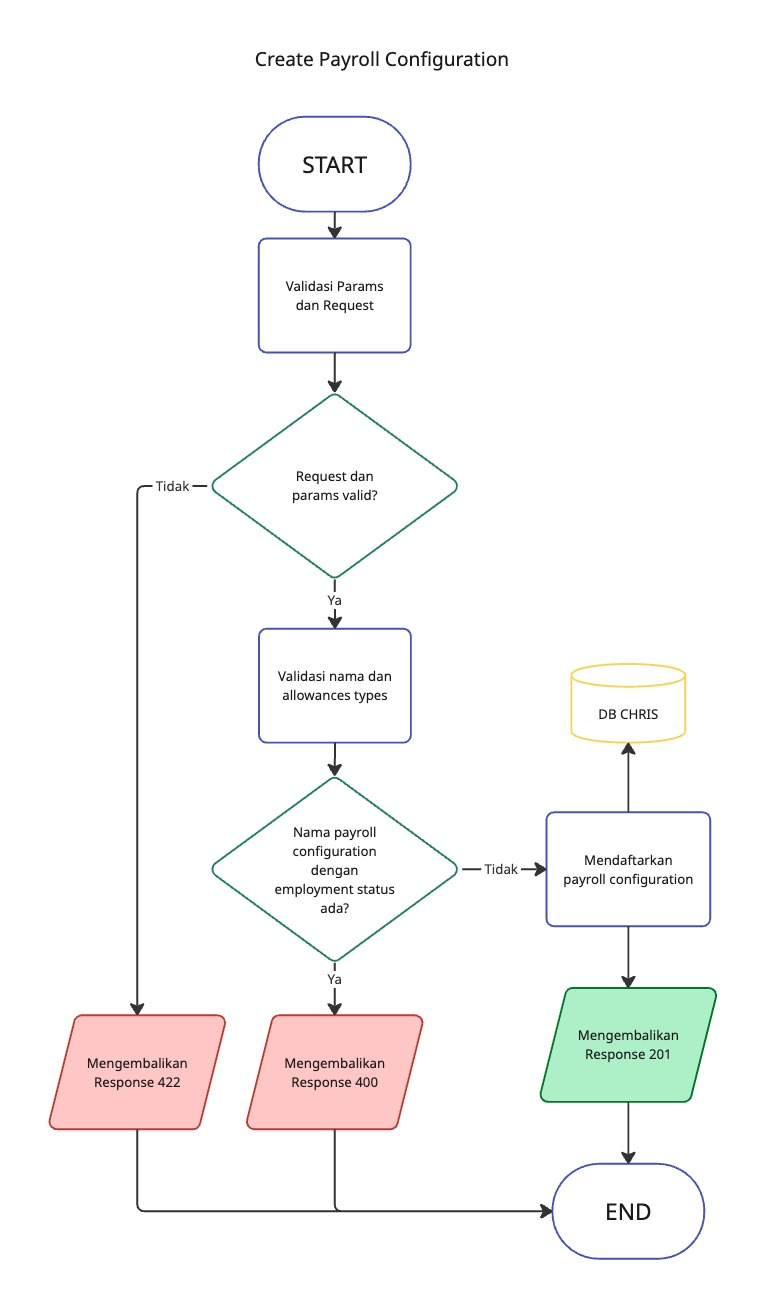
\includegraphics[width=0.8\textwidth]{assets/pics/payroll-config-create.jpg}}
    \caption{\textit{Flowchart create payroll configuration}}
    \label{fig:create_payroll_config}
\end{figure}

\begin{figure}[H]
    \centering
    \fbox{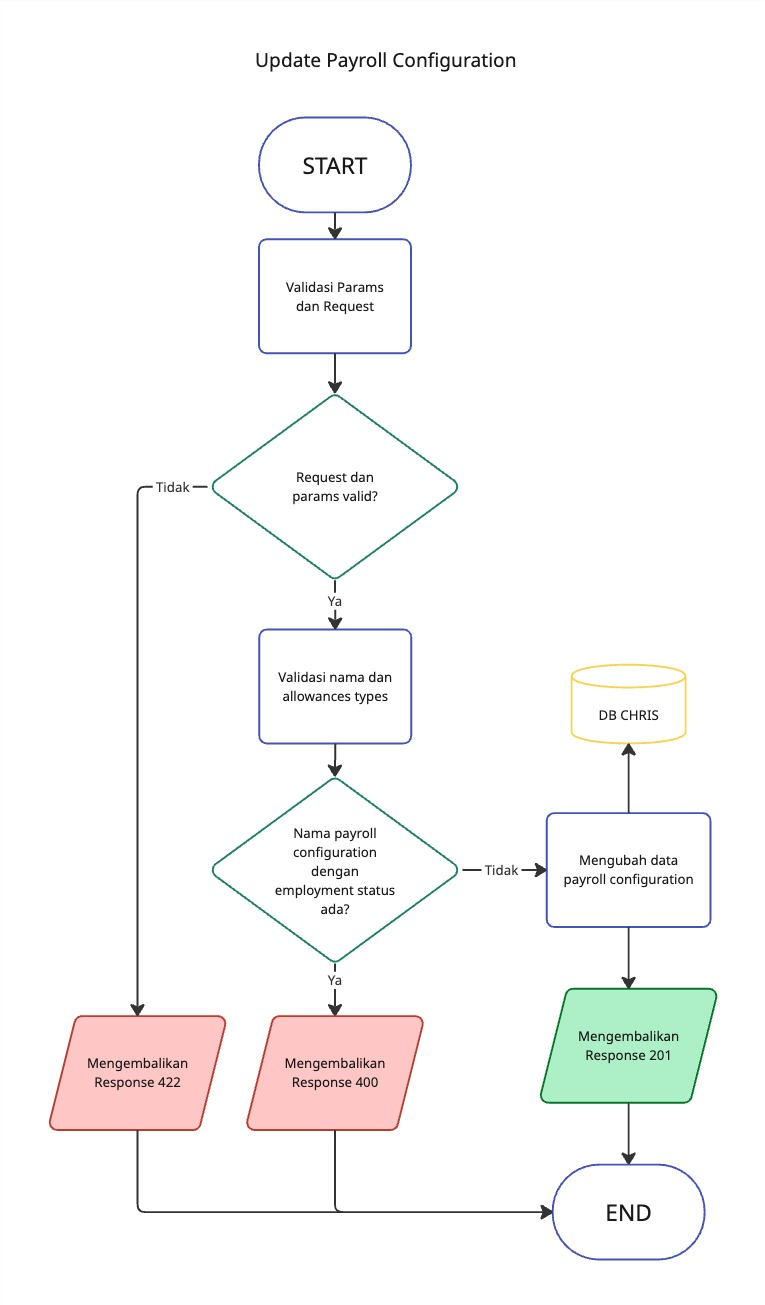
\includegraphics[width=0.8\textwidth]{assets/pics/payroll-config-update.jpg}}
    \caption{\textit{Flowchart update payroll configuration}}
    \label{fig:update_payroll_config}
\end{figure}

\begin{figure}[H]
    \centering
    \fbox{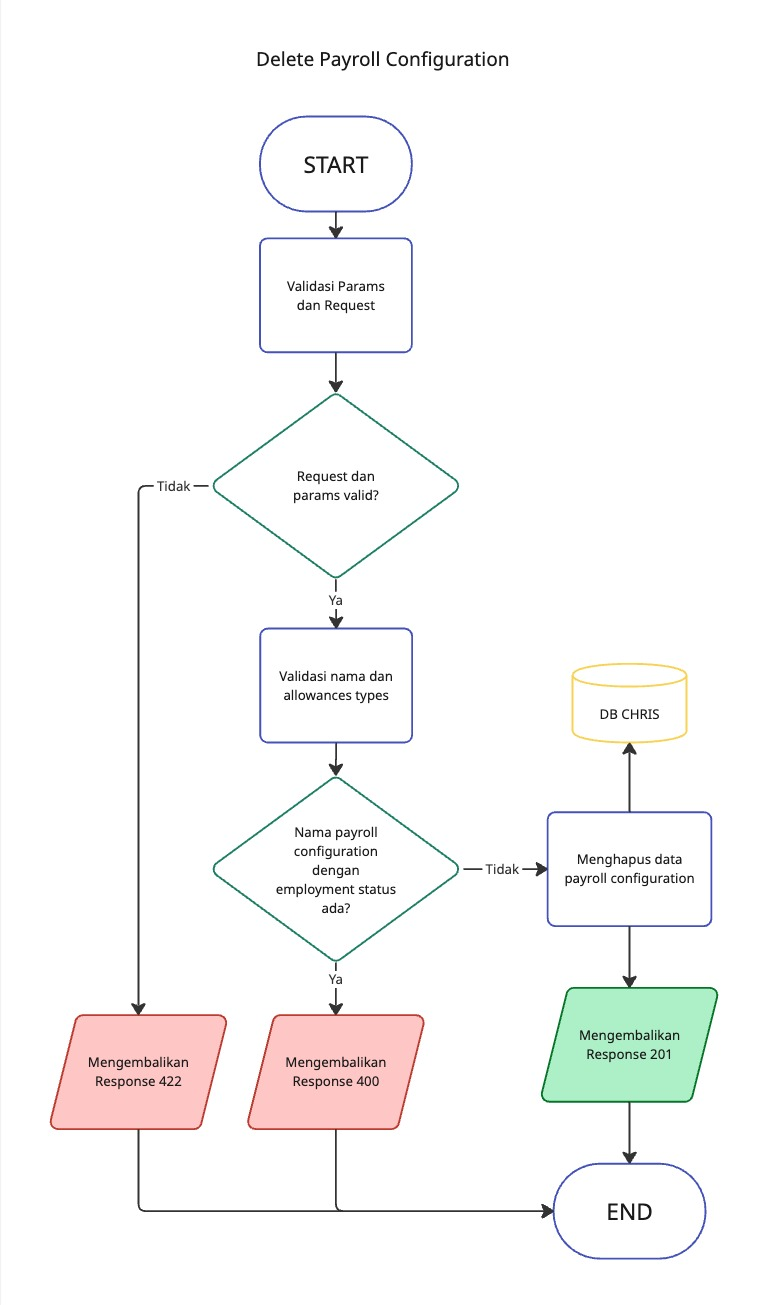
\includegraphics[width=0.8\textwidth]{assets/pics/payroll-config-delete.jpg}}
    \caption{\textit{Flowchart delete payroll configuration}}
    \label{fig:delete_payroll_config}
\end{figure}

Gambar \ref{fig:create_payroll_config}, \ref{fig:update_payroll_config}, dan \ref{fig:delete_payroll_config} menggambarkan alur proses pembuatan, pengubahan, dan penghapusan data \textit{Payroll Configuration}. Ketiga proses tersebut menerapkan validasi yang sama, yaitu pengecekan \textit{request} dan \textit{params}, dan pengecekan terhadap kombinasi nama Payroll Configuration dan Employment\textit{ Status} yang sudah terdaftar sebelumnya.

Apabila \textit{request} atau \textit{parameter} yang dikirimkan tidak sesuai dengan format atau aturan yang telah ditentukan, sistem akan merespons dengan kode 422 (\textit{Invalid Format}) sebagai penolakan terhadap permintaan yang tidak valid. Selain itu, jika kombinasi nama \textit{Payroll Configuration} dan \textit{Employment Status} telah terdaftar sebelumnya, sistem akan mengembalikan respons kode 400 (\textit{Bad Request}) untuk mencegah terjadinya duplikasi data.

Validasi ini bertujuan untuk menjaga konsistensi dan integritas data dalam sistem. Jika seluruh validasi berhasil dilewati, maka proses pembuatan, pengubahan, atau penghapusan akan dilanjutkan, dengan sistem memberikan respons berupa kode 201 (Created) untuk pembuatan, serta kode 200 (OK) untuk pengubahan dan penghapusan data.

% ----------------------%
\paragraph{User Allowances}
% ----------------------%
Setelah \textit{Superadmin} membuat \textit{payroll configuration}, langkah selanjutnya adalah mengatur data gaji setiap pegawai. Proses ini dilakukan melalui modul \textit{User Management}, di mana \textit{Superadmin} memilih \textit{Payroll Configuration} berdasarkan status kepegawaian pengguna, mengisi besaran gaji pokok, serta melengkapi jumlah masing-masing tunjangan yang ditetapkan. 

% -------------------- %
\begin{figure}[H]
    \centering
    \fbox{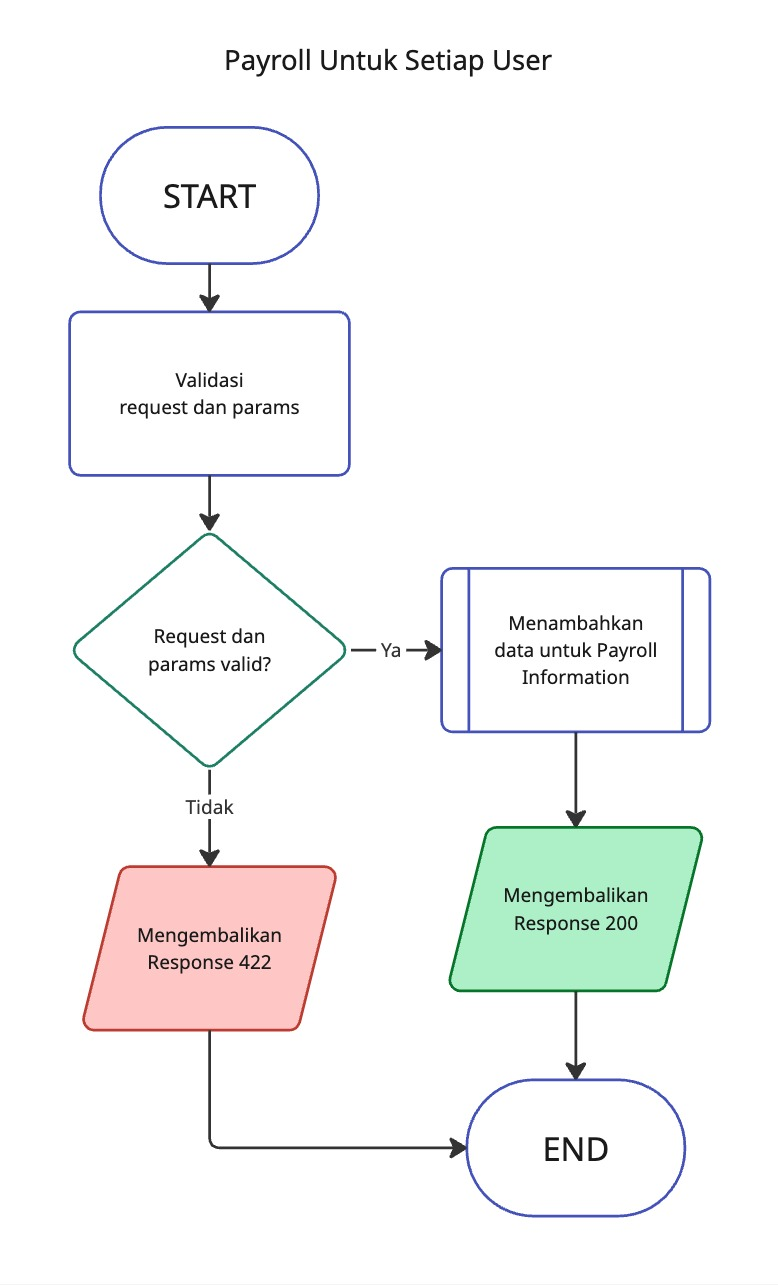
\includegraphics[height=0.7\textheight]{assets/pics/payroll-untuk-setiap-user.jpg}}
    \caption{\textit{Flowchart} implementasi payroll untuk setiap user}
    \label{fig:payroll_untuk_setiap_user}
\end{figure}

Gambar \ref{fig:payroll_untuk_setiap_user} menunjukkan proses untuk validasi \textit{request} dan \textit{parameter} akan dilanjuti dengan proses menambahkan data untuk \textit{payroll information} secara \textit{general}.

% -------------------- %
\begin{figure}[H]
    \centering
    \fbox{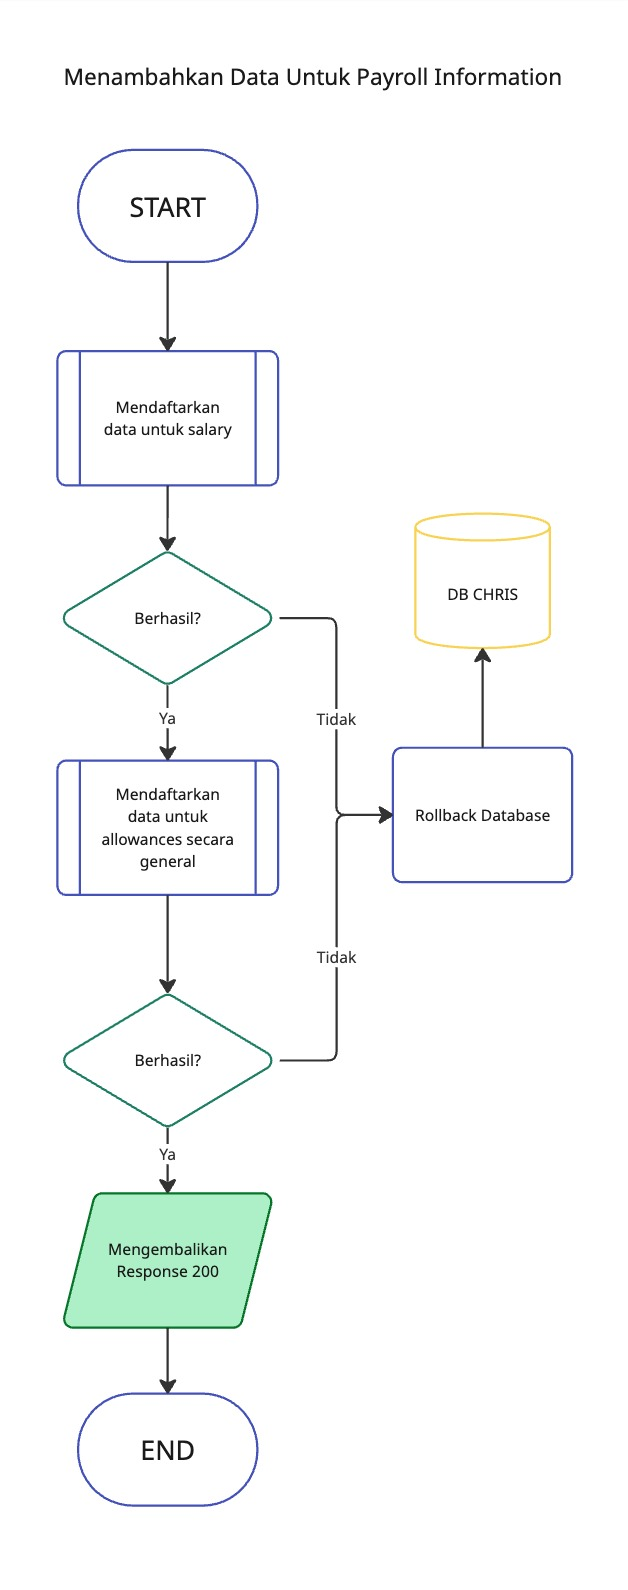
\includegraphics[height=0.7\textheight]{assets/pics/menambahkan-data-untuk-payroll-information.jpg}}
    \caption{\textit{Flowchart} menambahkan data untuk payroll information}
    \label{fig:menambahkan_data_payroll_information}
\end{figure}

Pada \textit{user management}, terdapat suatu field bernama \textit{Payroll Information} yang berisi data gaji pegawai, dan field untuk memilih \textit{Payroll Configuration} yang telah dibuat sebelumnya. Setelah memilih \textit{Payroll Configuration}, \textit{Superadmin} dapat mengisi data gaji pokok, tunjangan, dan potongan yang berlaku untuk pegawai tersebut. Gambar \ref{fig:payroll_untuk_setiap_user} menunjukkan alur sistem untuk pembuatan data gaji pegawai.

% -------------------- %
\begin{figure}[H]
    \centering
    \fbox{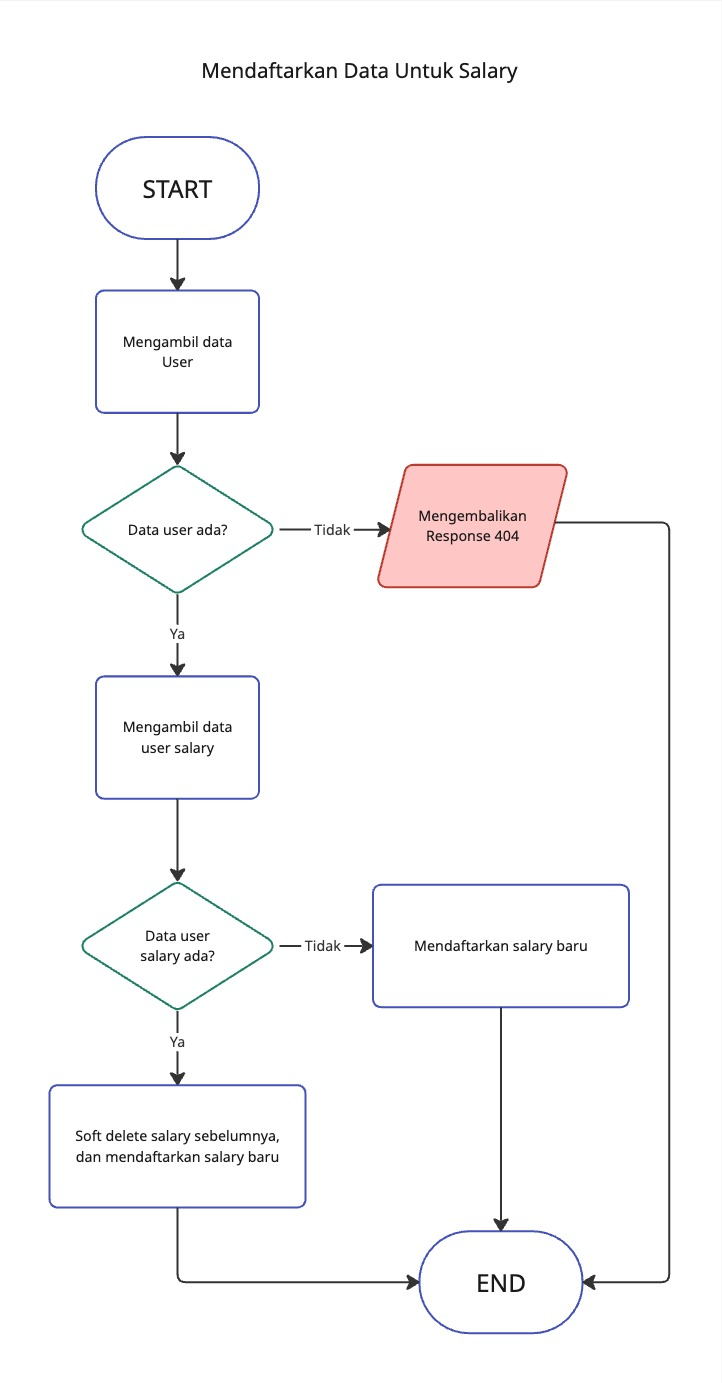
\includegraphics[height=0.7\textheight]{assets/pics/mendaftarkan-data-untuk-salary.jpg}}
    \caption{\textit{Flowchart} mendaftarkan data untuk salary}
    \label{fig:mendaftarkan_data_untuk_salary}
\end{figure}

Gambar \ref{fig:mendaftarkan_data_untuk_salary} menunjukkan proses pembuatan data gaji pegawai yang dimulai dengan mencari data pegawai dan mengambil data gaji pegawai tersebut. Setelah itu, jika data tersebut ditemukan, sistem akan menghapus data gaji pegawai yang lama secara \textit{soft delete} dan membuat data gaji pegawai yang baru.
% -------------------- %
\begin{figure}[H]
    \centering
    \fbox{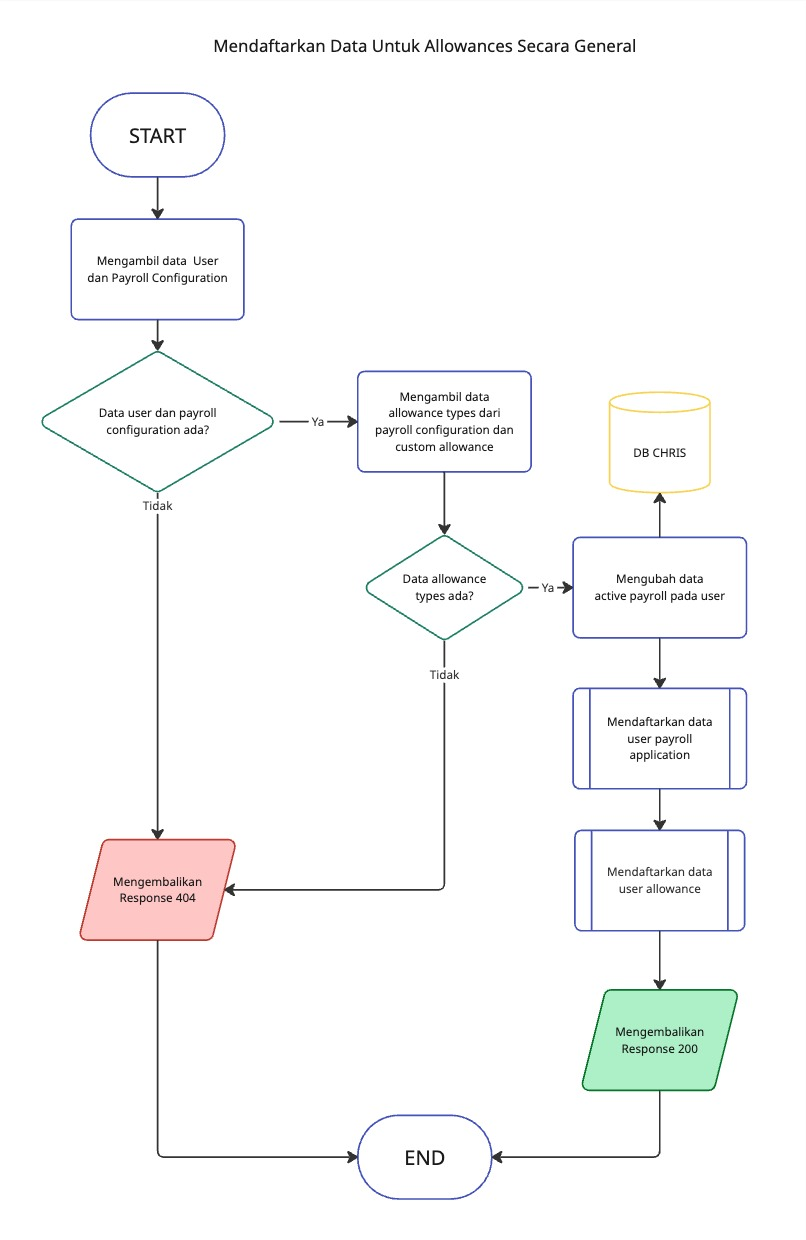
\includegraphics[height=0.6\textheight]{assets/pics/mendaftarkan-data-untuk-allowances-secara-general.jpg}}
    \caption{\textit{Flowchart} mendaftarkan data user allowances secara \textit{general}}
    \label{fig:mendaftarkan_data_user_allowances_secara_general}
\end{figure}

Gambar \ref{fig:mendaftarkan_data_user_allowances_secara_general} menggambarkan alur proses pendaftaran data tunjangan pegawai secara umum. Proses ini diawali dengan pengambilan data pegawai dan \textit{Payroll Configuration} yang telah tersedia. Selanjutnya, sistem mengekstraksi daftar tunjangan yang tercantum dalam \textit{Payroll Configuration} tersebut. Setelah itu, sistem akan memperbarui informasi \textit{Active Payroll} pada data pegawai, dan mendaftarkan entri baru pada \textit{User Payroll Application} guna menghubungkan pegawai dengan konfigurasi payroll yang aktif. Terakhir, sistem akan mendaftarkan data \textit{User Allowances} beserta nominal masing-masing tunjangan dan potongan yang telah ditentukan sebelumnya.

% -------------------- %
\begin{figure}[H]
    \centering
    \fbox{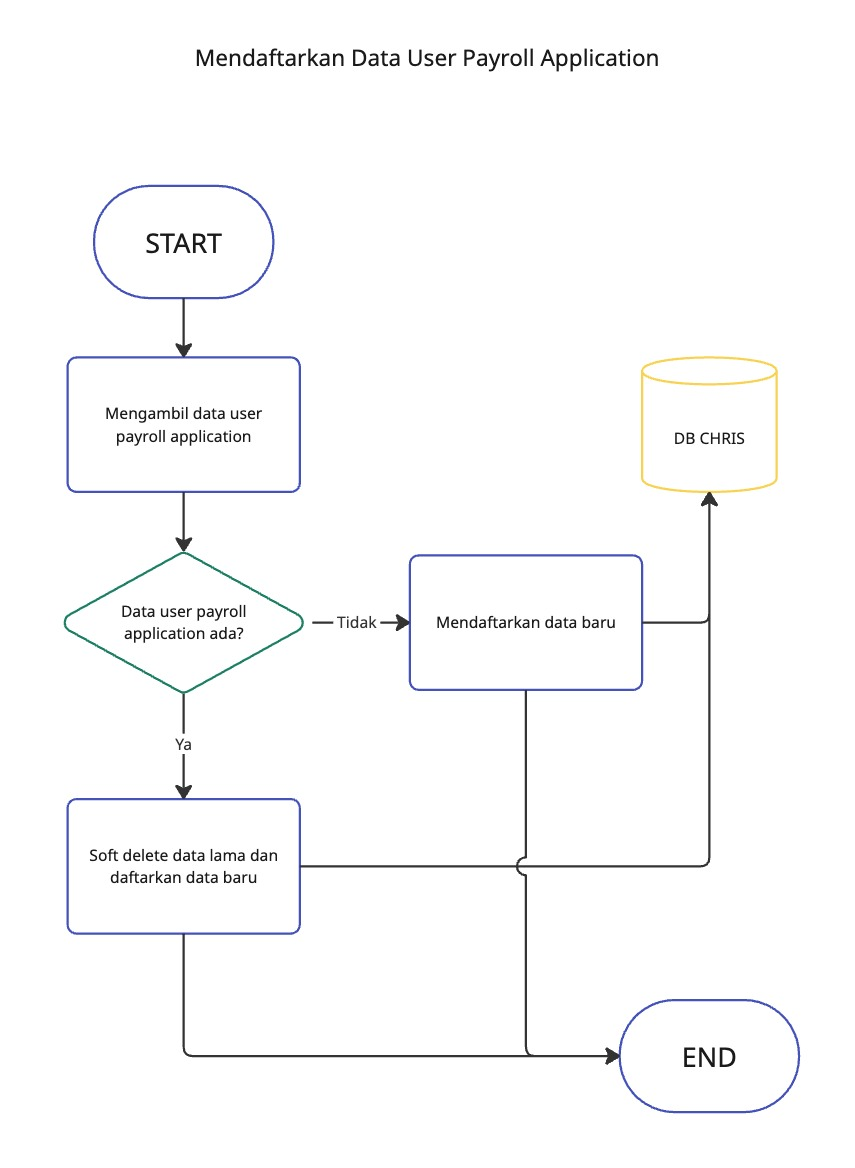
\includegraphics[height=0.8\textheight]{assets/pics/mendaftarkan-data-user-payroll-application.jpg}}
    \caption{\textit{Flowchart} mendaftarkan data \textit{user payroll application}}
    \label{fig:mendaftarkan_data_user_payroll_application}
\end{figure}

Gambar \ref{fig:mendaftarkan_data_user_payroll_application} menggambarkan proses pendaftaran data \textit{User Payroll Application} yang diawali dengan pencarian entri sebelumnya pada pegawai terkait. Jika tidak ditemukan, sistem akan langsung membuat entri baru pada tabel \textit{User Payroll Application}. Namun, apabila entri sudah ada, sistem akan terlebih dahulu melakukan \textit{soft delete} terhadap data tersebut, kemudian membuat entri baru guna memastikan hanya satu konfigurasi aktif yang tercatat untuk setiap pegawai. Pendekatan ini menjaga integritas historis tanpa menghapus data secara permanen.


% -------------------- %
\begin{figure}[H]
    \centering
    \fbox{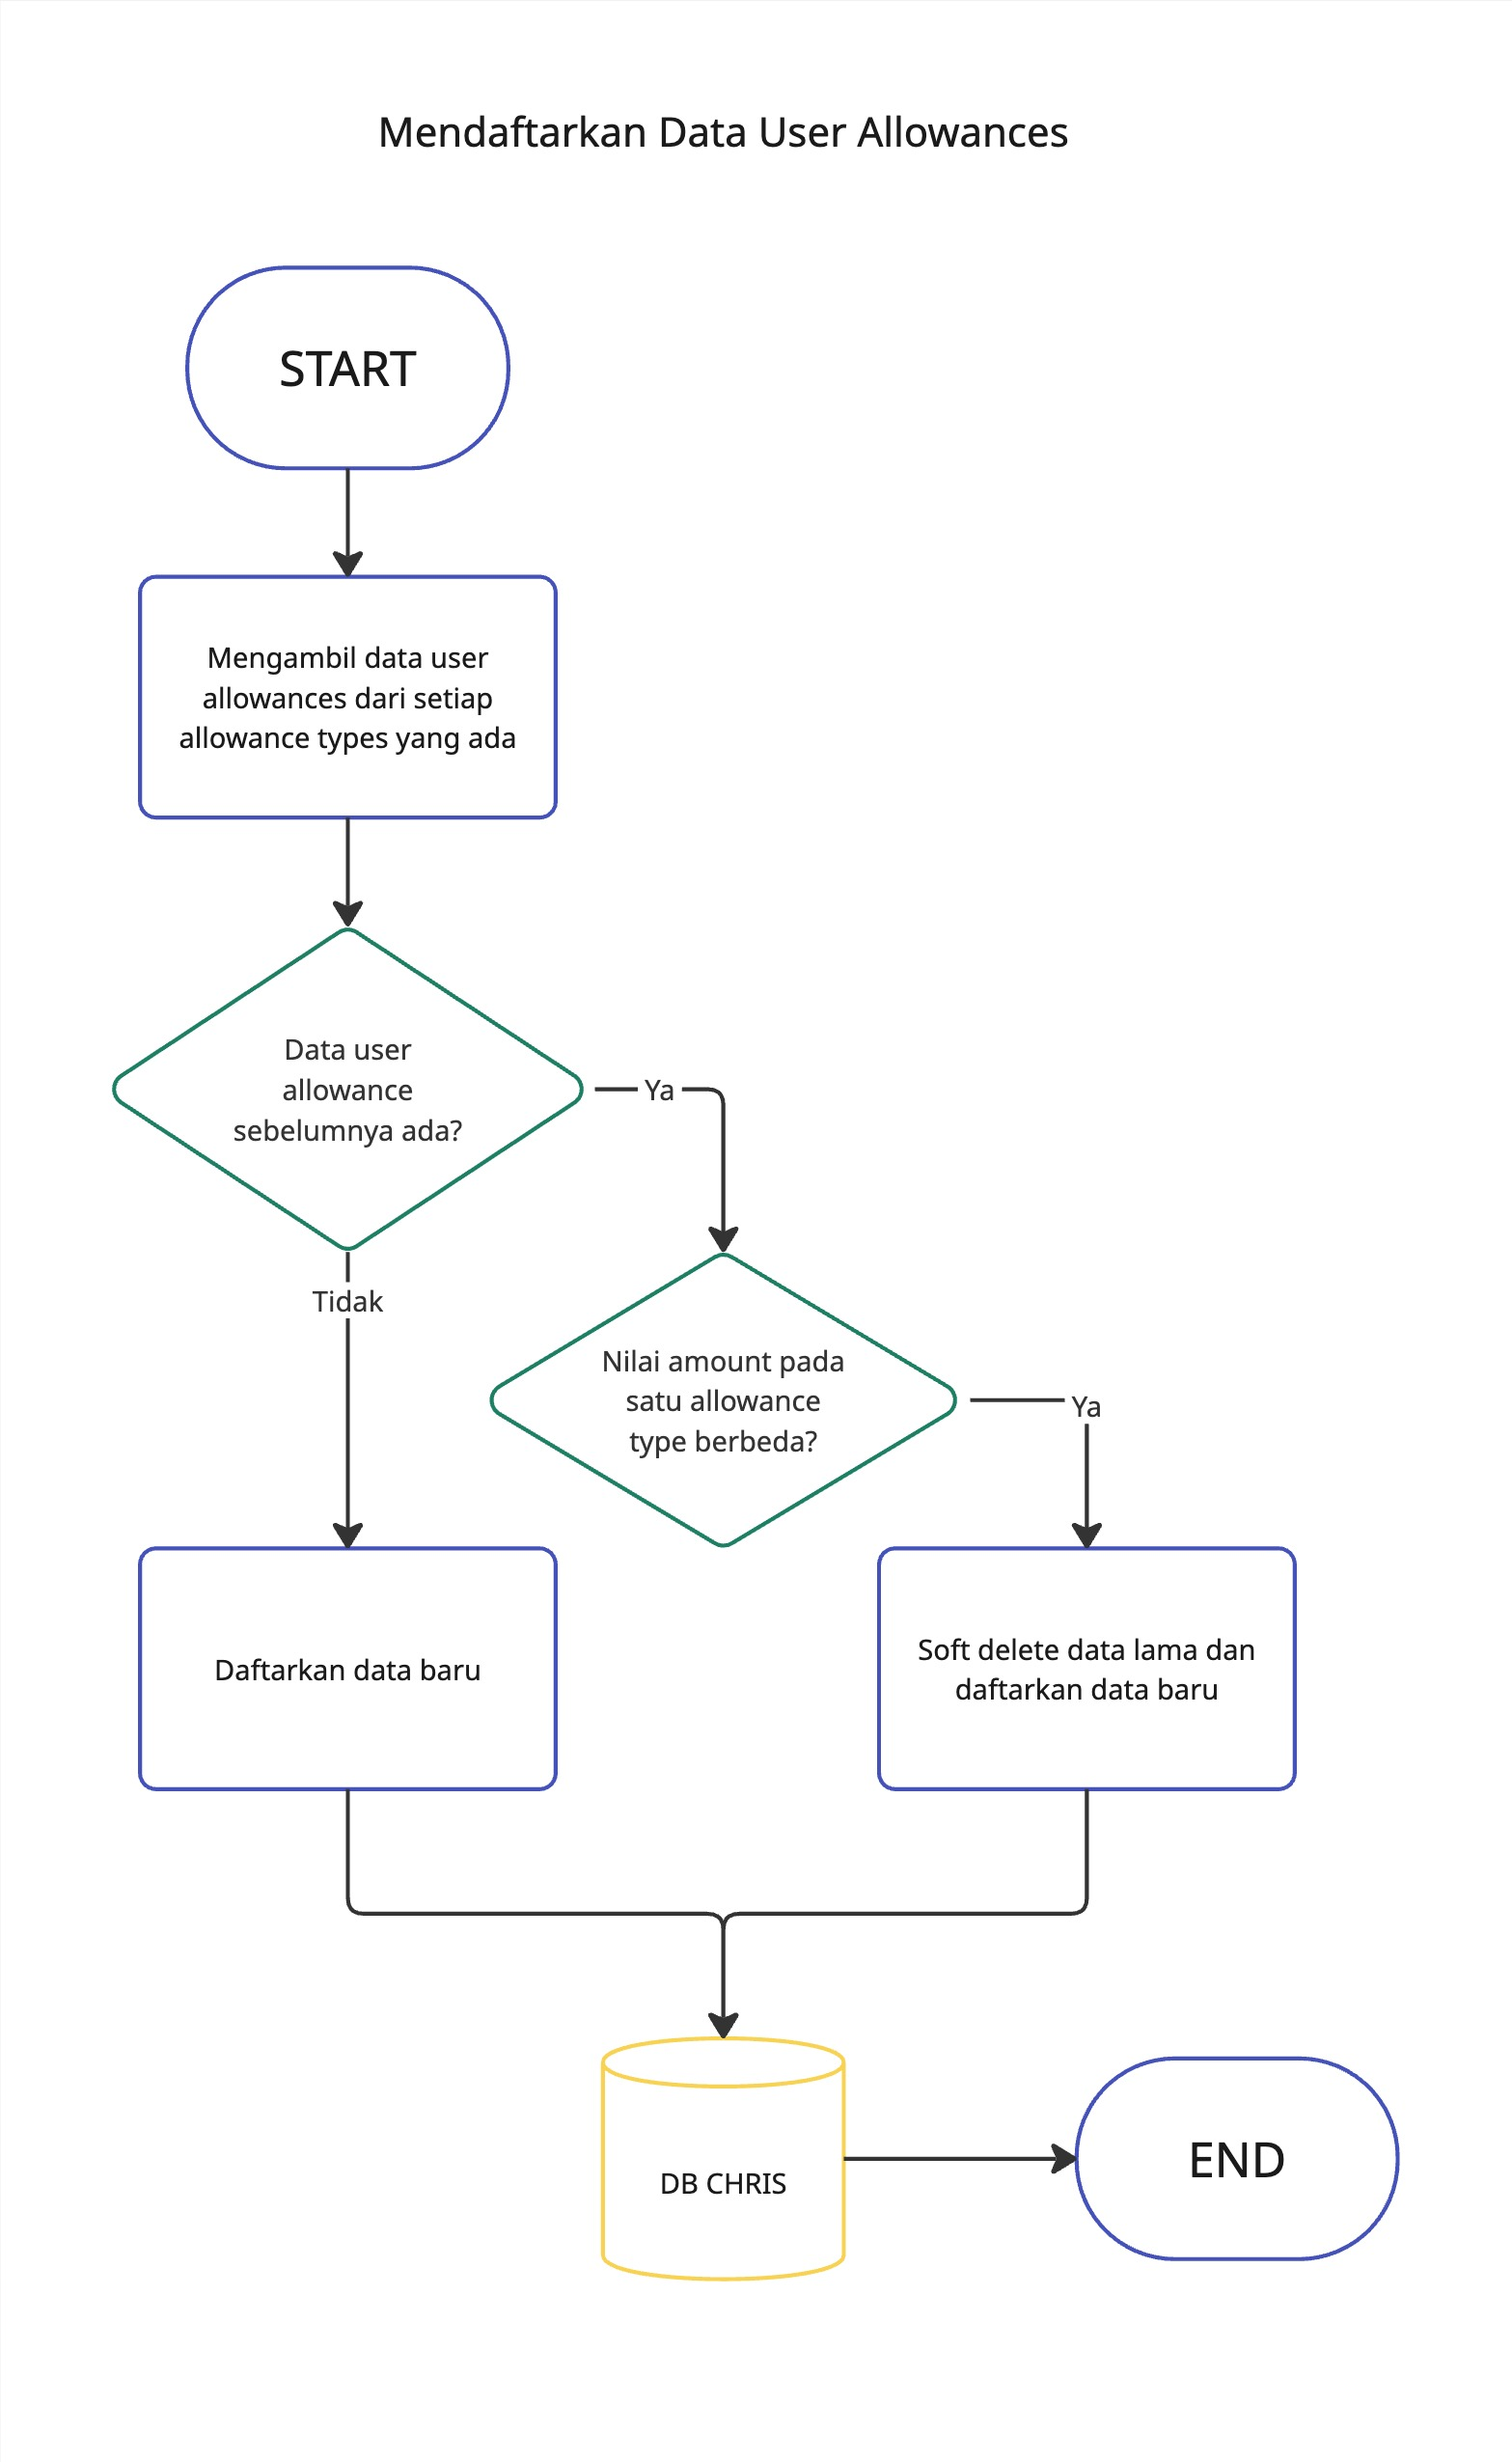
\includegraphics[height=0.7\textheight]{assets/pics/mendaftarkan-data-user-allowances.jpg}}
    \caption{\textit{Flowchart} mendaftarkan data \textit{user allowances}}
    \label{fig:mendaftarkan_data_user_allowances}
\end{figure}

Gambar \ref{fig:mendaftarkan_data_user_allowances} menggambarkan proses pendaftaran data tunjangan pegawai yang diawali dengan pencarian data \textit{User Allowances} berdasarkan setiap \textit{Allowance Type} yang dimiliki pegawai. Apabila data tidak ditemukan, sistem akan membuat entri baru dengan mengisikan \textit{Allowance Type} beserta nominal tunjangan yang telah ditentukan. Namun, jika data ditemukan, sistem akan melakukan pengecekan terhadap kesesuaian nominal tunjangan. Jika nominal yang ditemukan sama, maka tidak ada perubahan yang dilakukan. Sebaliknya, jika terdapat perbedaan, sistem akan memperbarui nilai nominal dengan yang baru, serta melakukan \textit{soft delete} pada data lama. Pendekatan ini diterapkan untuk menjaga riwayat data dan memungkinkan pelacakan perubahan secara historis.

% -------------------- %
% SALARY SLIP
\paragraph{Salary Slip}
% -------------------- %
Setelah data gaji pegawai selesai dibuat, \textit{Superadmin} dapat mengakses modul \textit{Salary Slip} untuk melakukan finalisasi gaji. Proses finalisasi ini memungkinkan pengecekan akhir terhadap rincian gaji sebelum tanggal gajian. Di PT Ganda Visi Jayatama, proses penggajian dilakukan setiap tanggal 25, sehingga proses finalisasi disarankan dilakukan pada tanggal 24 setiap bulannya. Setelah tanggal 25, data tidak dapat lagi diubah.
\begin{figure}[H]
    \centering
    \fbox{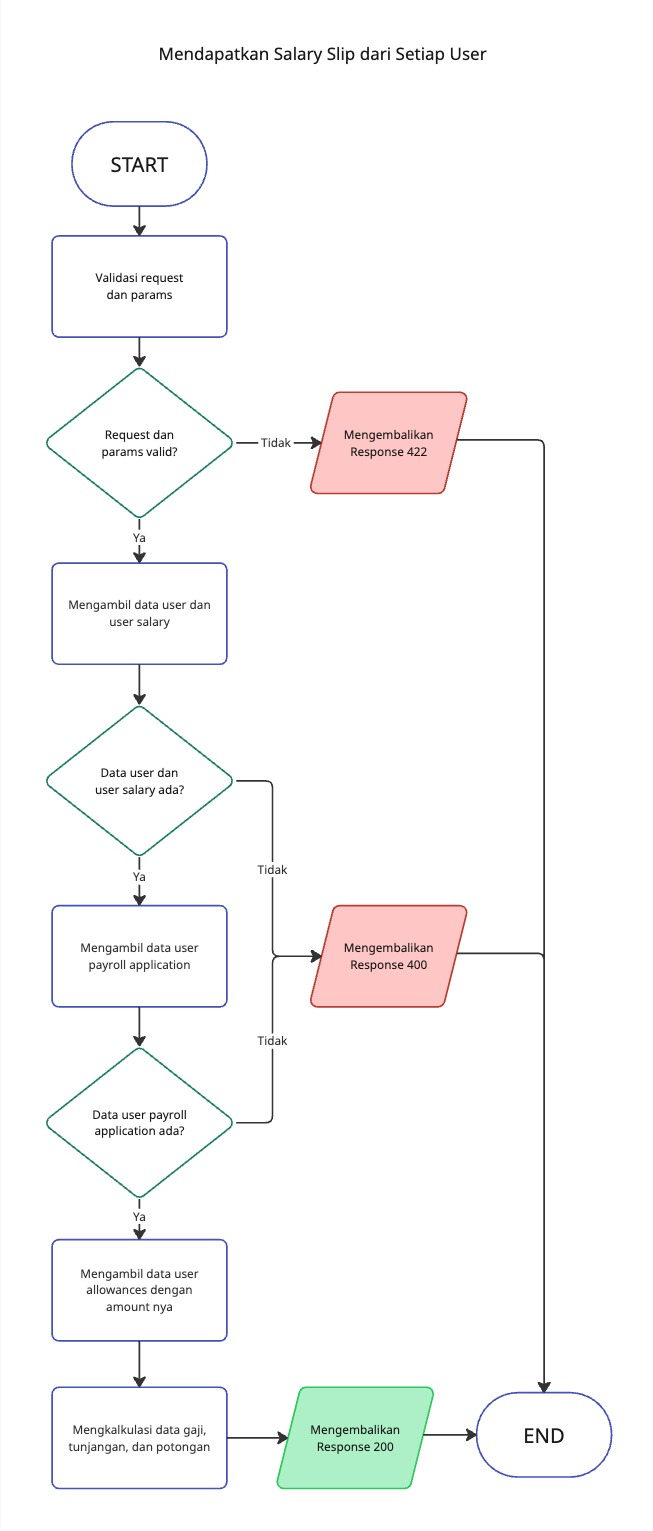
\includegraphics[height=0.8\textheight]{assets/pics/mendapatkan-salary-slip-dari-setiap-user.jpg}}
    \caption{\textit{Flowchart} mendapatkan salary slip dari setiap user}
    \label{fig:mendapatkan_salary_slip_dari_setiap_user}
\end{figure}

Gambar \ref{fig:mendapatkan_salary_slip_dari_setiap_user} menunjukkan proses mendapatkan slip gaji pegawai yang dimulai dengan mencari data pegawai berdasarkan \textit{Payroll Configuration} yang telah dibuat sebelumnya. Setelah itu, sistem akan mengambil data gaji pegawai, tunjangan-tunjangan yang telah dibuatkan sebelumnya, dan membuat slip gaji berdasarkan data tersebut. 

Untuk pegawai yang telah memiliki data gaji terverifikasi, mereka dapat melihat slip gaji mereka masing-masing pada halaman \textit{Salary Slip} dan mengunduhnya dalam format PDF. Hal ini memungkinkan pegawai untuk mengakses informasi gaji mereka secara transparan dan mudah.

Untuk mendapatkan slip gaji historis, sistem akan terlebih dahulu menentukan periode waktu berdasarkan tanggal yang diminta, yaitu awal hingga akhir bulan tersebut. Setelah itu, sistem akan mencari seluruh entri data gaji (\textit{User Salary}) yang memiliki tanggal pembuatan (\textit{created\_at}) sebelum atau sama dengan akhir periode, dan belum dihapus atau dihapus setelah periode tersebut berakhir. Seluruh data yang ditemukan kemudian diurutkan berdasarkan tanggal pembuatan dari yang terbaru ke yang terlama. Dari hasil pengurutan tersebut, sistem akan memilih satu entri data gaji paling terbaru yang masih berlaku pada periode tersebut. Entri tersebut kemudian digunakan untuk mengambil informasi tunjangan (\textit{User Allowances}) dan pemotongan berdasarkan konfigurasi yang berlaku, lalu disusun menjadi slip gaji pegawai.

% ---------------------------------- %
\subsection{Leave Permit}
Modul \textit{Leave Permit} merupakan fitur yang memungkinkan pegawai untuk mengajukan cuti dan atasan untuk menyetujui atau menolak permohonan tersebut. Modul ini dirancang untuk mencerminkan alur persetujuan yang realistis dan terstruktur, dengan mempertimbangkan hierarki jabatan dalam perusahaan. Modul ini juga mencakup fitur-fitur seperti pagination, pengelolaan jenis cuti, dan sistem notifikasi untuk memastikan proses pengajuan cuti berjalan dengan lancar.

Sistem ini sudah pernah digunakan sebelumnya, namun mengalami beberapa kendala yang perlu diperbaiki. Beberapa perbaikan yang dilakukan antara lain adalah:
\begin{itemize}
    \item \textbf{Refactor Form Submission}: Proses pengajuan cuti ditambahkan \textit{officer in charge} (\textit{oic}) dengan tujuan sebagai pengganti pegawai saat ia cuti.
    \item \textbf{Cancel Button}: Ditambahkan fitur pembatalan (\textit{cancel}) pengajuan cuti, sehingga pegawai dapat membatalkan permohonan yang belum disetujui.
    \item \textbf{Leave Permit Dashboard}: Tampilan daftar cuti ditampilkan di \textit{home page} supaya semua pegawai dapat melihat siapa saja yang mengajukan cuti di minggu itu.
\end{itemize}


\subsection{Sistem Hierarki Supervisi}
Sistem CHRIS\@ menerapkan struktur hierarki berbasis pohon (\textit{tree hierarchy}) untuk mengelola hubungan antara pegawai dan atasan. Modul-modul dalam sistem ini, seperti pengajuan cuti, bergantung pada struktur tersebut, di mana permohonan cuti hanya dapat disetujui oleh atasan langsung dari pegawai yang bersangkutan.

Dengan implementasi tree hierarchy, setiap pegawai dapat memiliki lebih dari satu atasan yang terhubung dalam rantai struktural. Hal ini memungkinkan sistem untuk secara efisien menentukan pihak yang berwenang dalam proses persetujuan, penolakan, serta pengelolaan data pegawai. Pendekatan ini juga membantu menciptakan struktur organisasi yang lebih fleksibel dan terintegrasi. Fungsi ini juga dapat digunakan untuk modul-modul yang lain yang memerlukan pengelolaan hubungan antar pegawai.

\subsection{User Management dan Validasi Data}
Sistem CHRIS\@ telah dilengkapi dengan modul \textit{User Management} yang berfungsi untuk mengelola data pegawai secara efisien. Modul ini mencakup fitur untuk menambahkan, memperbarui, dan menghapus data pegawai, serta melakukan validasi terhadap input yang diberikan melalui formulir. Validasi ini bertujuan untuk memastikan bahwa data yang dimasukkan sesuai dengan format dan ketentuan yang berlaku. Meskipun demikian, terdapat beberapa aspek yang perlu disempurnakan guna meningkatkan integritas data dan kemudahan pengelolaan.

Adapun sejumlah perbaikan yang telah dilakukan meliputi:
\begin{itemize}
    \item \textbf{Refactor User Management}: Alur pengelolaan data pegawai diperbarui agar setiap pegawai memiliki status kepegawaian yang jelas, serta agar proses pengelolaannya menjadi lebih terstruktur dan mudah diakses.
    \item \textbf{Validasi Form Input}: Validasi pada form input ditingkatkan untuk mencegah kesalahan dalam pengisian data, seperti format email yang tidak valid, nomor telepon yang tidak sesuai, atau bidang yang wajib diisi namun terlewatkan.
    \item \textbf{Penyempurnaan Struktur Tabel}: Struktur tabel \textit{user} dan \texttt{employment\_status} disempurnakan untuk meningkatkan konsistensi dan integritas data, sekaligus memudahkan proses pengolahan dan pencarian informasi.
\end{itemize}

Sebelumnya, status kepegawaian (\textit{employment status}) masih didefinisikan secara \textit{hardcoded} melalui enumerasi di dalam sistem. Kini, status tersebut telah dipisahkan ke dalam tabel tersendiri yang lebih dinamis dan fleksibel. Perubahan ini dilakukan sebagai bagian dari penerapan praktik terbaik dalam pengembangan sistem, sekaligus menjadi sarana pembelajaran untuk memahami alur kerja sistem backend secara lebih mendalam.





\section{Implementasi Sistem}
% ---------------------------------- %
\subsection{Implementasi \textit{Payroll}}
\subsubsection{API \textit{Endpoints}}
\subsubsection{Contoh \textit{Request} dan \textit{Response}}

\subsection{Implementasi \textit{Leave Permit}}
\subsubsection{API \textit{Endpoints}}
\subsubsection{Contoh \textit{Request} dan \textit{Response}}




% -------------------- %
% -------------------- %
% -------------------- %
% -------------------- %
% -------------------- %
% -------------------- %
% -------------------- %
% -------------------- %
% -------------------- %
% -------------------- %
% ini cmd + enter
\clearpage
.
\clearpage
.
\clearpage
% -------------------- %
% -------------------- %
% -------------------- %
% -------------------- %
% -------------------- %
% -------------------- %
% -------------------- %
% -------------------- %
% -------------------- %
% -------------------- %


% \begin{figure}
%      \centering
%      \begin{subfigure}[b]{0.3\textwidth}
%          \centering
%          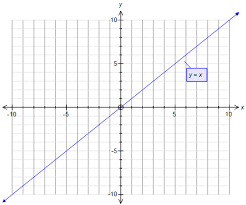
\includegraphics[width=\textwidth]{assets/pics/graph1.png}
%          \caption{$y=x$}
%          \label{fig:y equals x}
%      \end{subfigure}
%      \hfill
%      \begin{subfigure}[b]{0.3\textwidth}
%          \centering
%          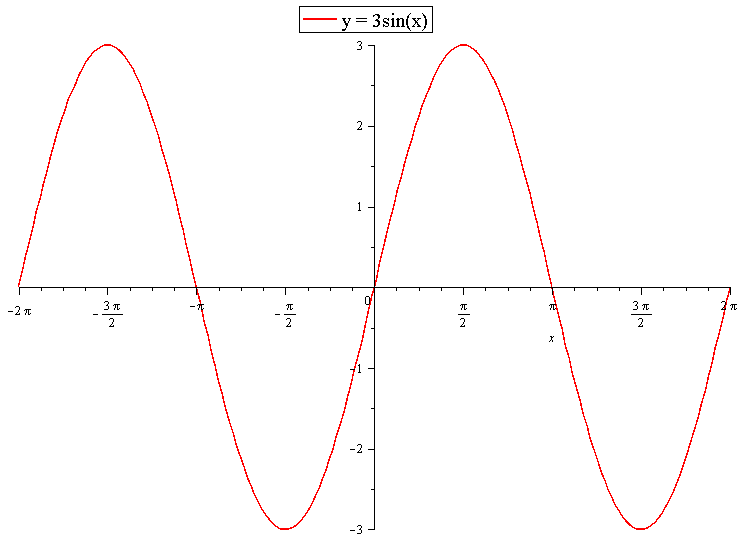
\includegraphics[width=\textwidth]{assets/pics/graph2.png}
%          \caption{$y=3sinx$}
%          \label{fig:three sin x}
%      \end{subfigure}
%      \hfill
%      \begin{subfigure}[b]{0.3\textwidth}
%          \centering
%          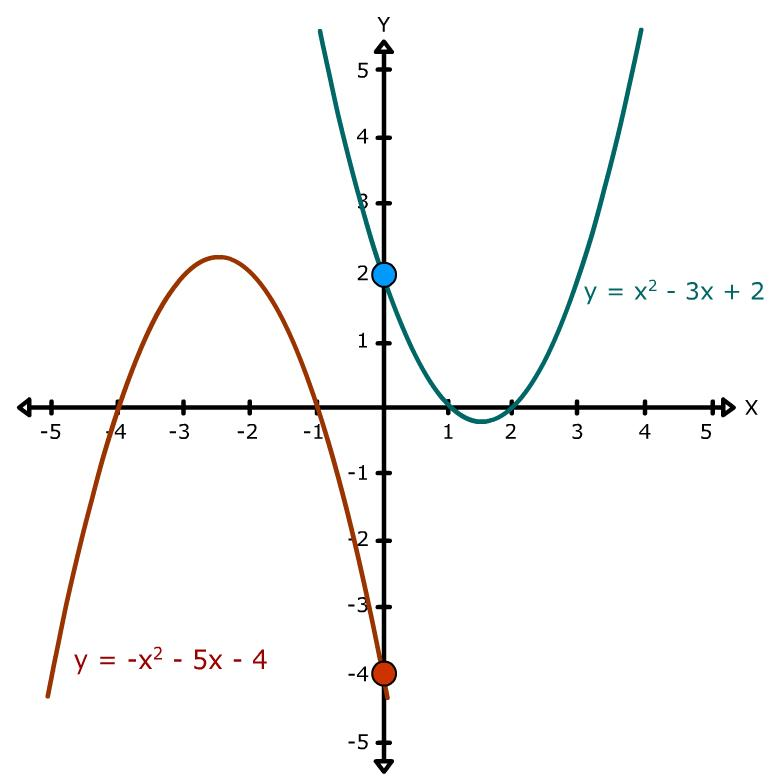
\includegraphics[width=\textwidth]{assets/pics/graph3.jpg}
%          \caption{$y=5/x$}
%          \label{fig:five over x}
%      \end{subfigure}
%         \caption{Three simple graphs}
%         \label{fig:three graphs}
% \end{figure}
% \subsubsection{Subsub-section}

\paragraph{Paragraph 1}

Contoh Python script yang digunakan dapat dilihat pada Kode \ref{kode1}.

{\footnotesize
\begin{lstlisting}[basicstyle=\linespread{0.8},language=Python, caption= Contoh potongan kode, label= kode1]
import numpy as np
    
def incmatrix(genl1,genl2):
    m = len(genl1)
    n = len(genl2)
    M = None #to become the incidence matrix
    VT = np.zeros((n*m,1), int)  #dummy variable
    
    #compute the bitwise xor matrix
    M1 = bitxormatrix(genl1)
    M2 = np.triu(bitxormatrix(genl2),1) 

    for i in range(m-1):
        for j in range(i+1, m):
            [r,c] = np.where(M2 == M1[i,j])
            for k in range(len(r)):
                VT[(i)*n + r[k]] = 1;
                VT[(i)*n + c[k]] = 1;
                VT[(j)*n + r[k]] = 1;
                VT[(j)*n + c[k]] = 1;
                
                if M is None:
                    M = np.copy(VT)
                else:
                    M = np.concatenate((M, VT), 1)
                
                VT = np.zeros((n*m,1), int)
    
    return M
\end{lstlisting}
}

\subparagraph{Sub-paragraph 1.1}

\lipsum[17-18]

\subparagraph{Sub-paragraph 1.2}

\lipsum[19-20]

\subsubsection{Subsub-section}

\lipsum[21-22]

\paragraph{Paragraph}

\subparagraph{Sub-paragraph}

\subparagraph{Sub-paragraph}

\subsection{Sub-section}

\lipsum[25-26]

\section{Section}

\subsection{Sub-Section}

\subsubsection{Sub-sub-section}

\paragraph{Paragraph}

\subparagraph{Sub-paragraph}

\lipsum[27]

\paragraph{Paragraph}

\subparagraph{Sub-paragraph}
\subparagraph{Sub-paragraph}


\section{Kendala dan Solusi yang Ditemukan}